\documentclass[11pt,a4paper]{article}

\usepackage[utf8]{inputenc}
\usepackage{amsmath}
\usepackage{booktabs}
\usepackage{graphicx}
\usepackage[margin=0.95in]{geometry}
\usepackage{natbib}
\usepackage{url}

\graphicspath{{../outputs/figures/}}
\linespread{1.2}

% Single Source of Truth: auto-generated numeric macros from src/energiewende/reporting.py
% Auto-generated by src/energiewende/reporting.py — DO NOT EDIT BY HAND
\newcommand{\DECapShareThirteen}{67.0}
\newcommand{\DECapShareTwentyThree}{52.5}
\newcommand{\DEGenShareThirteen}{74.0}
\newcommand{\DEGenShareTwentyThree}{57.1}
\newcommand{\DEGenShareDelta}{-16.9}
\newcommand{\DECapTopTwentyThree}{18.8}
\newcommand{\DEGenTopTwentyThree}{22.5}
\newcommand{\DERenElecThirteen}{25.3}
\newcommand{\DERenElecTwentyThree}{51.9}
\newcommand{\DECapConnTwentyThreeGW}{22.8}
\newcommand{\DECapDecommTwentyOneGW}{11.1}
\newcommand{\BalEUGenMedTwentyThree}{59.6}
\newcommand{\BigSixGenMedTwentyThree}{42.1}
\newcommand{\DEBigSixGenRankTwentyThree}{2}
\newcommand{\DEGasRetThirteen}{825}
\newcommand{\DEGasRetTwentyOne}{979}
\newcommand{\DEGasRetTwentyThree}{973}
\newcommand{\DEGasTwhTwentyOne}{698.2}
\newcommand{\DEGasTwhTwentyThree}{552.2}
\newcommand{\DEDensityThirteen}{1.28}
\newcommand{\DEDensityTwentyOne}{1.40}
\newcommand{\DEDensityTwentyThree}{1.76}
\newcommand{\DECrisisDenomSharePct}{102.7}
\newcommand{\DECrisisGasDropPct}{20.9}
\newcommand{\DEGasConcThirteen}{26.0}
\newcommand{\DEGasConcTwentyThree}{13.3}
\newcommand{\BigSixGasConcMedTwentyThree}{70.1}
\newcommand{\DEElecEurTwentyOne}{0.321}
\newcommand{\DEElecEurTwentyThree}{0.407}
\newcommand{\DEElecPpsTwentyThree}{0.364}
\newcommand{\DEElecTaxTwentyOne}{50.9}
\newcommand{\DEElecTaxTwentyThree}{28.1}
\newcommand{\DEElecExTaxTwentyOne}{0.158}
\newcommand{\DEElecExTaxTwentyThree}{0.293}
\newcommand{\DEGasEurTwentyOne}{0.067}
\newcommand{\DEGasEurTwentyThree}{0.119}
\newcommand{\DEWarmTotalTwentyOne}{3.3}
\newcommand{\DEWarmTotalTwentyThree}{8.2}
\newcommand{\EUWarmTotalMedTwentyThree}{7.1}
\newcommand{\DEWarmTotalRankTwentyOne}{17}
\newcommand{\DEWarmTotalRankTwentyThree}{10}
\newcommand{\DEWarmLowIncTwentyOne}{7.8}
\newcommand{\DEWarmLowIncTwentyThree}{14.3}
\newcommand{\DEArrearsLowIncTwentyOne}{6.5}
\newcommand{\DEArrearsLowIncTwentyThree}{9.3}
\newcommand{\MOneCoef}{-0.533}
\newcommand{\MOnePval}{0.008}
\newcommand{\MOneWithinR}{0.071}
\newcommand{\MTwoCoef}{-0.539}
\newcommand{\MThreeCoef}{0.0007}
\newcommand{\MThreePval}{0.024}


\title{Market Structure, Affordability, and Social Resilience in Germany's Energiewende (2013--2023):\\ A Comparative European Panel Analysis}
\author{Islam Md Monaim}
\date{November 2026}

\begin{document}
\maketitle

\begin{abstract}
\noindent
This study evaluates how Germany's decade-long energy transition interacted with electricity and gas market concentration, household energy affordability, and thermal energy poverty across 36 European economies from 2013 to 2023, integrating eight official Eurostat datasets. Four findings emerge. First, Germany doubled its renewable electricity share (\DERenElecThirteen\% to \DERenElecTwentyThree\%) while reducing cumulative electricity generation concentration by \DEGenShareDelta~percentage points (\DEGenShareThirteen\% to \DEGenShareTwentyThree\%), yet peer-cohort selection reverses Germany's comparative standing: Germany sits near the balanced EU-27 median (\BalEUGenMedTwentyThree\%) but ranks \#\DEBigSixGenRankTwentyThree~of~6 (second-most concentrated) among Europe's Big-6 large markets (median \BigSixGenMedTwentyThree\%). Second, exact log-decomposition reveals that \DECrisisDenomSharePct\% of Germany's 2021--2023 jump in gas-retailer density (\DEDensityTwentyOne~to \DEDensityTwentyThree~retailers/TWh) was a denominator artifact driven by a \DECrisisGasDropPct\% crisis collapse in gas consumption rather than retailer entry; the cleaner concentration metric (\texttt{GRTL\_NG5}) confirms genuine retail fragmentation (\DEGasConcThirteen\% to \DEGasConcTwentyThree\%, lowest in the Big-6). Third, abolishing the EEG levy nearly halved Germany's electricity tax wedge (\DEElecTaxTwentyOne\% to \DEElecTaxTwentyThree\%), yet an ex-tax surge (\DEElecExTaxTwentyOne~to \DEElecExTaxTwentyThree~EUR/kWh) pushed household electricity to \DEElecEurTwentyThree~EUR/kWh. Fourth, Germany's inability to keep homes adequately warm more than doubled (\DEWarmTotalTwentyOne\% to \DEWarmTotalTwentyThree\%, crossing above the EU-27 median of \EUWarmTotalMedTwentyThree\%), hitting \DEWarmLowIncTwentyThree\% among low-income households. Two-way fixed effects regressions subject to a strict 100\% leave-one-out stability gate confirm that renewable expansion robustly tracks power deconcentration ($\hat{\beta}=\MOneCoef$, $p=\MOnePval$) and lower concentration tracks modestly lower PPS electricity prices ($\hat{\beta}=\MThreeCoef$, $p=\MThreePval$), whereas direct market-to-poverty links fail the gate---demonstrating that market structure alone does not replace targeted social buffers during supply shocks.
\end{abstract}

\section{Introduction}

Evaluating Germany's \emph{Energiewende} requires connecting three domains that are too often studied in isolation: \emph{market structure} (whether renewable buildout dilutes incumbent dominance), \emph{household affordability} (how wholesale shocks and policy tax wedges shape retail bills), and \emph{social resilience} (whether households—especially low-income groups—experience rising thermal deprivation during external energy shocks).

This paper extends an earlier descriptive market-structure note into a unified, reproducible four-pillar empirical framework covering 36 European economies over 2013--2023. Every statistic and table in this manuscript is auto-generated from verified Eurostat API extracts via a single programmatic pipeline (\texttt{python -m energiewende.pipeline}), preventing transcription drift between code and text. All regressions are strictly non-causal within-country associations screened by a pre-registered 100\% leave-one-country-out stability gate.

\section{Data, Provenance, and Measurement}

We integrate eight official Eurostat sources: energy market indicators (\texttt{nrg\_ind\_market}) \citep{eurostat2026market}, simplified gas balances (\texttt{nrg\_bal\_s}) \citep{eurostat2026balances}, population (\texttt{demo\_pjan}) \citep{eurostat2026population}, renewable energy shares (\texttt{nrg\_ind\_ren}) \citep{eurostat2026ren}, bi-annual household electricity and gas prices including and excluding taxes (\texttt{nrg\_pc\_204}, \texttt{nrg\_pc\_202}) \citep{eurostat2026elecprice,eurostat2026gasprice}, and EU-SILC energy-poverty and utility-arrears surveys (\texttt{ilc\_mdes01}, \texttt{ilc\_mdes07}) \citep{eurostat2026warmth,eurostat2026arrears}. Variable definitions follow the EEA/Eurostat vocabulary \citep{eea2021indic} and are enforced via automated Germany-2013 unit checks and SHA-256 checksums in \texttt{data/manifest.json}.

Because unbalanced cross-country panels conflate real trends with smaller non-EU markets entering Eurostat reporting, we systematically compare Germany against three cohorts: (i)~all unbalanced reporters ($N \le 35$), (ii)~a constant balanced EU-27 cohort ($N=26$), and (iii)~Europe's Big-6 large interconnected markets (Germany, France, Italy, Spain, Poland, and the Netherlands).

\section{Pillar 1: Electricity Transition and Peer-Cohort Sensitivity}

Germany's renewable electricity share rose from \DERenElecThirteen\% in 2013 to \DERenElecTwentyThree\% in 2023, supported by \DECapConnTwentyThreeGW~GW of new capacity connected in 2023 alone and \DECapDecommTwentyOneGW~GW of legacy capacity decommissioned in 2021. Over the same decade, Germany's cumulative electricity generation share held by firms with at least 5\% of output fell from \DEGenShareThirteen\% to \DEGenShareTwentyThree\% (\DEGenShareDelta~pp), while capacity concentration dropped from \DECapShareThirteen\% to \DECapShareTwentyThree\% and the single largest firm's capacity share fell to \DECapTopTwentyThree\%.

Figure~\ref{fig:p1} demonstrates why benchmark cohort selection is decisive. Relative to all 35 unbalanced reporters, Germany appears below the median. Holding membership constant in the balanced EU-27 cohort places Germany close to the median (\BalEUGenMedTwentyThree\%). Against Europe's Big-6 large economies, however, Germany remains \emph{second-most concentrated} (rank \#\DEBigSixGenRankTwentyThree~of~6, substantially above the Big-6 median of \BigSixGenMedTwentyThree\%, behind only nuclear-incumbent France).

\begin{figure}[ht]
\centering
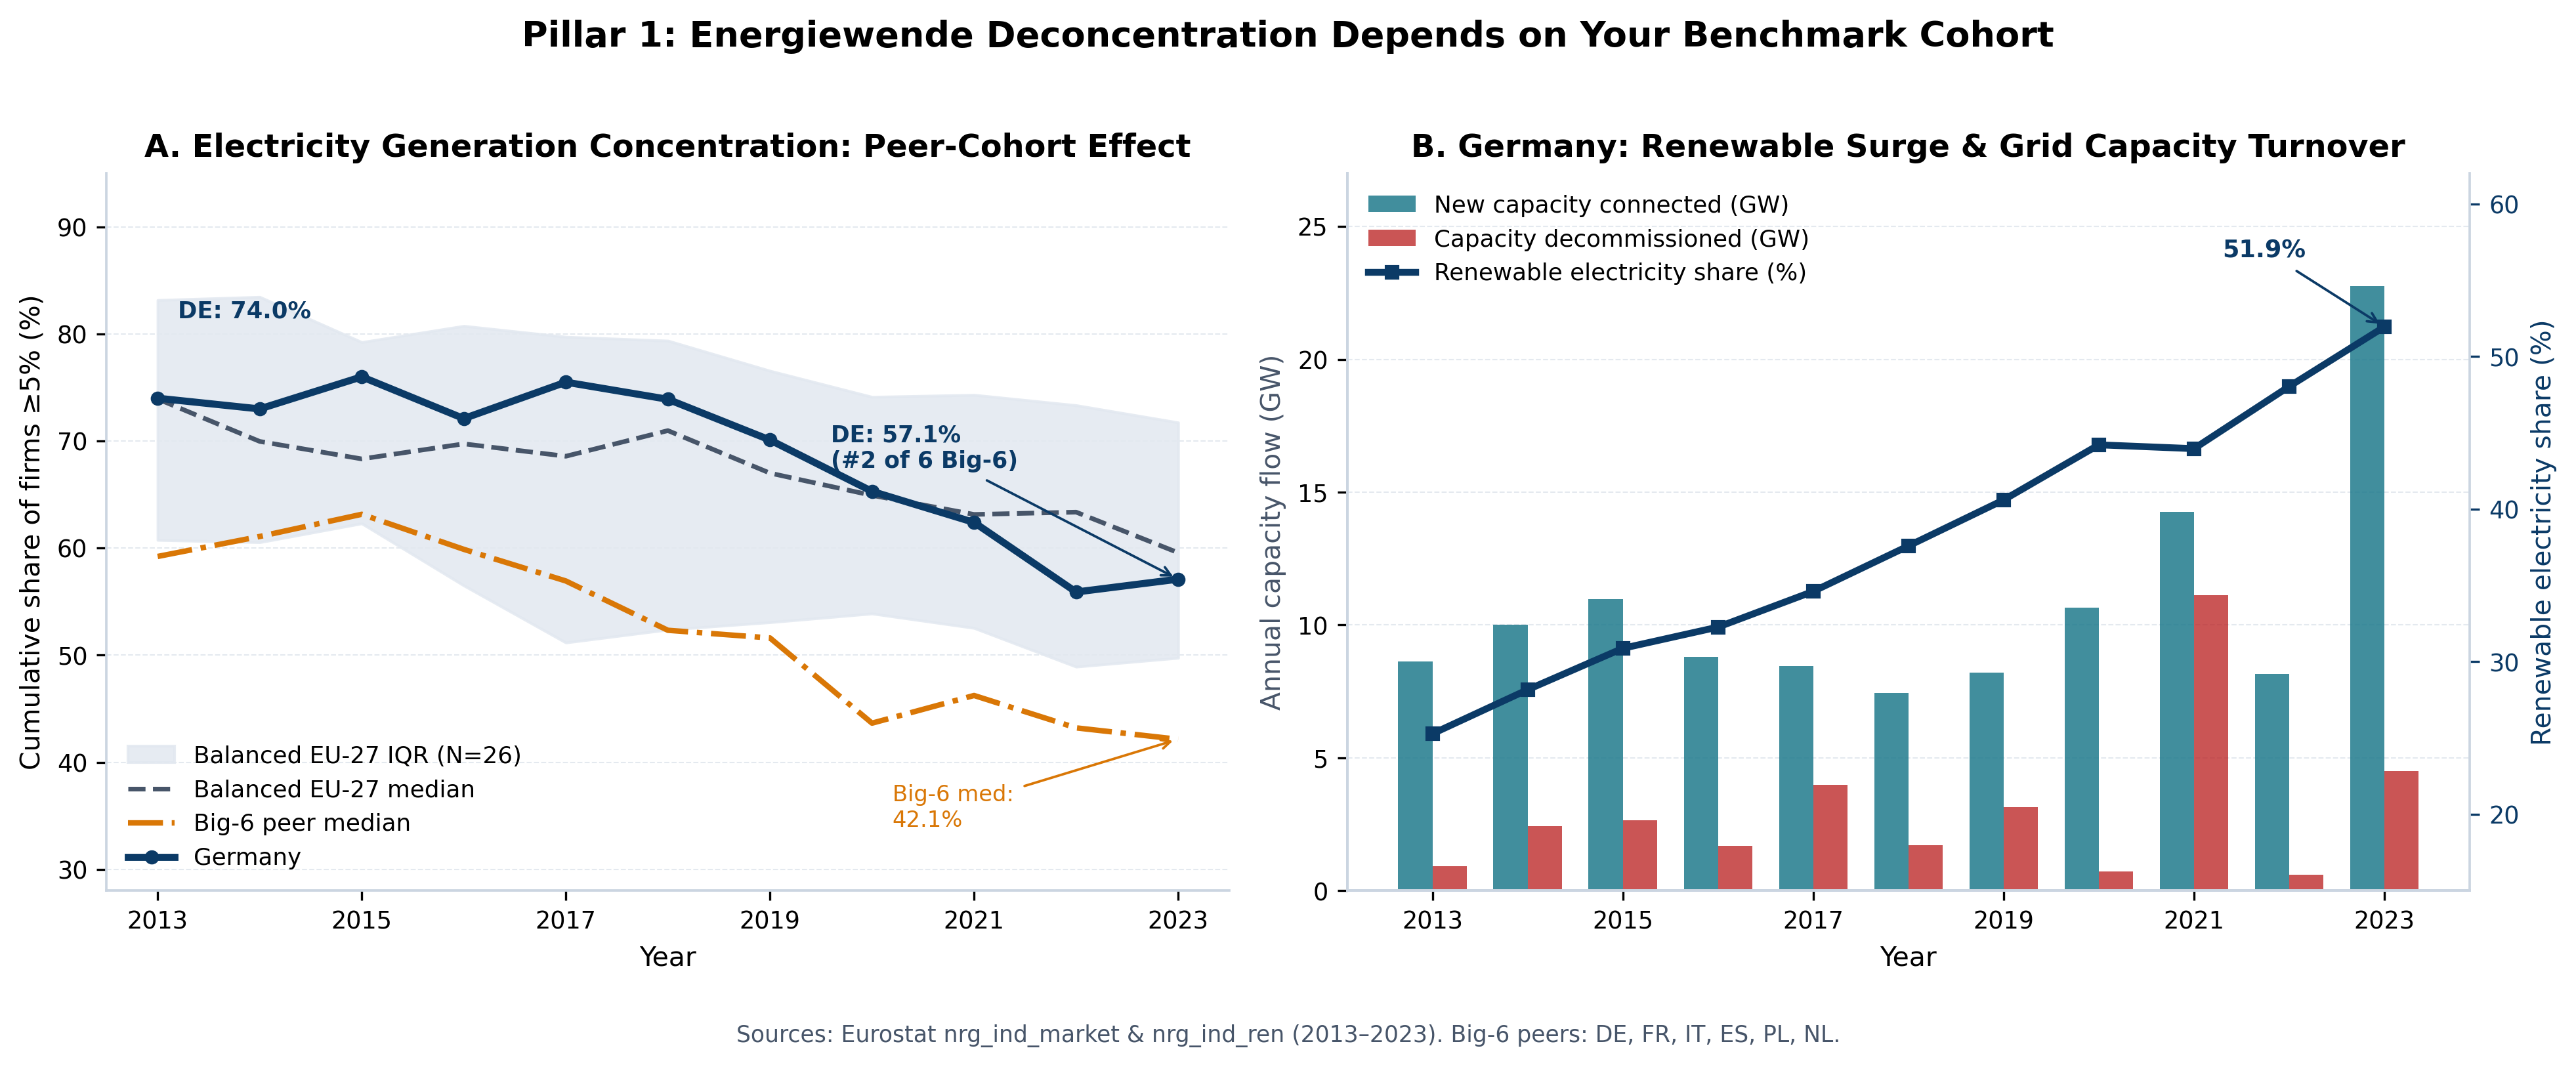
\includegraphics[width=0.98\textwidth]{fig1_electricity_transition_cohorts.png}
\caption{Pillar 1: Peer-cohort sensitivity in electricity generation concentration (Panel A) and Germany's renewable share and capacity turnover (Panel B). Sources: Eurostat \texttt{nrg\_ind\_market} and \texttt{nrg\_ind\_ren}, 2013--2023.}
\label{fig:p1}
\end{figure}

\section{Pillar 2: Gas Market Structure and Ratio Log-Decomposition}

Raw counts of gas retailers (\DEGasRetTwentyThree~in Germany in 2023) conflate market size. Scaling by final gas consumption (\texttt{retailers\_per\_twh}) raises Germany's metric from \DEDensityThirteen~(2013) to \DEDensityTwentyThree~(2023). However, exact log-decomposition of the ratio identity,
\begin{equation}
\Delta \ln\left(\frac{R_t}{C_t}\right) \equiv \Delta \ln(R_t) - \Delta \ln(C_t),
\end{equation}
exposes a severe crisis artifact (Table~\ref{tab:gas_decomp} and Figure~\ref{fig:p2}). While genuine retailer entry drove density growth during 2013--2017, between 2021 and 2023 German retailer counts actually edged \emph{down} (\DEGasRetTwentyOne~to \DEGasRetTwentyThree) even as density jumped from \DEDensityTwentyOne~to \DEDensityTwentyThree. Exactly \DECrisisDenomSharePct\% of that log surge came from the \DECrisisGasDropPct\% collapse in German final gas demand (\DEGasTwhTwentyOne~to \DEGasTwhTwentyThree~TWh). By contrast, the share-based concentration indicator (\texttt{GRTL\_NG5}) avoids demand-shock distortion and confirms deep structural fragmentation: Germany's major gas retailers ($\ge 5\%$ share) declined from \DEGasConcThirteen\% to \DEGasConcTwentyThree\%—far below the Big-6 median of \BigSixGasConcMedTwentyThree\%.

\begin{table}[ht]
\centering
\caption{Exact log-decomposition of Germany's gas-retailer density (\texttt{GRTL} / TWh)}
\label{tab:gas_decomp}
\resizebox{\textwidth}{!}{%
\begin{tabular}{@{}lrrrrrr@{}}
\toprule
Regime & Retailers $\Delta$\% & Gas TWh $\Delta$\% & Density $\Delta$\% & Entry ($\Delta\ln R$) & Demand ($-\Delta\ln C$) & Demand share \\
\midrule
Full decade (2013-2023) & +17.9\% & -14.1\% & +37.3\% & +0.165 & +0.152 & 47.9\% \\
Entry expansion (2013-2017) & +20.6\% & +0.2\% & +20.4\% & +0.187 & -0.002 & -1.0\% \\
Pre-crisis plateau (2017-2021) & -1.6\% & +8.5\% & -9.3\% & -0.016 & -0.081 & 83.4\% \\
Energy crisis shock (2021-2023) & -0.6\% & -20.9\% & +25.7\% & -0.006 & +0.235 & 102.7\% \\
\bottomrule
\end{tabular}}
\end{table}


\begin{figure}[ht]
\centering
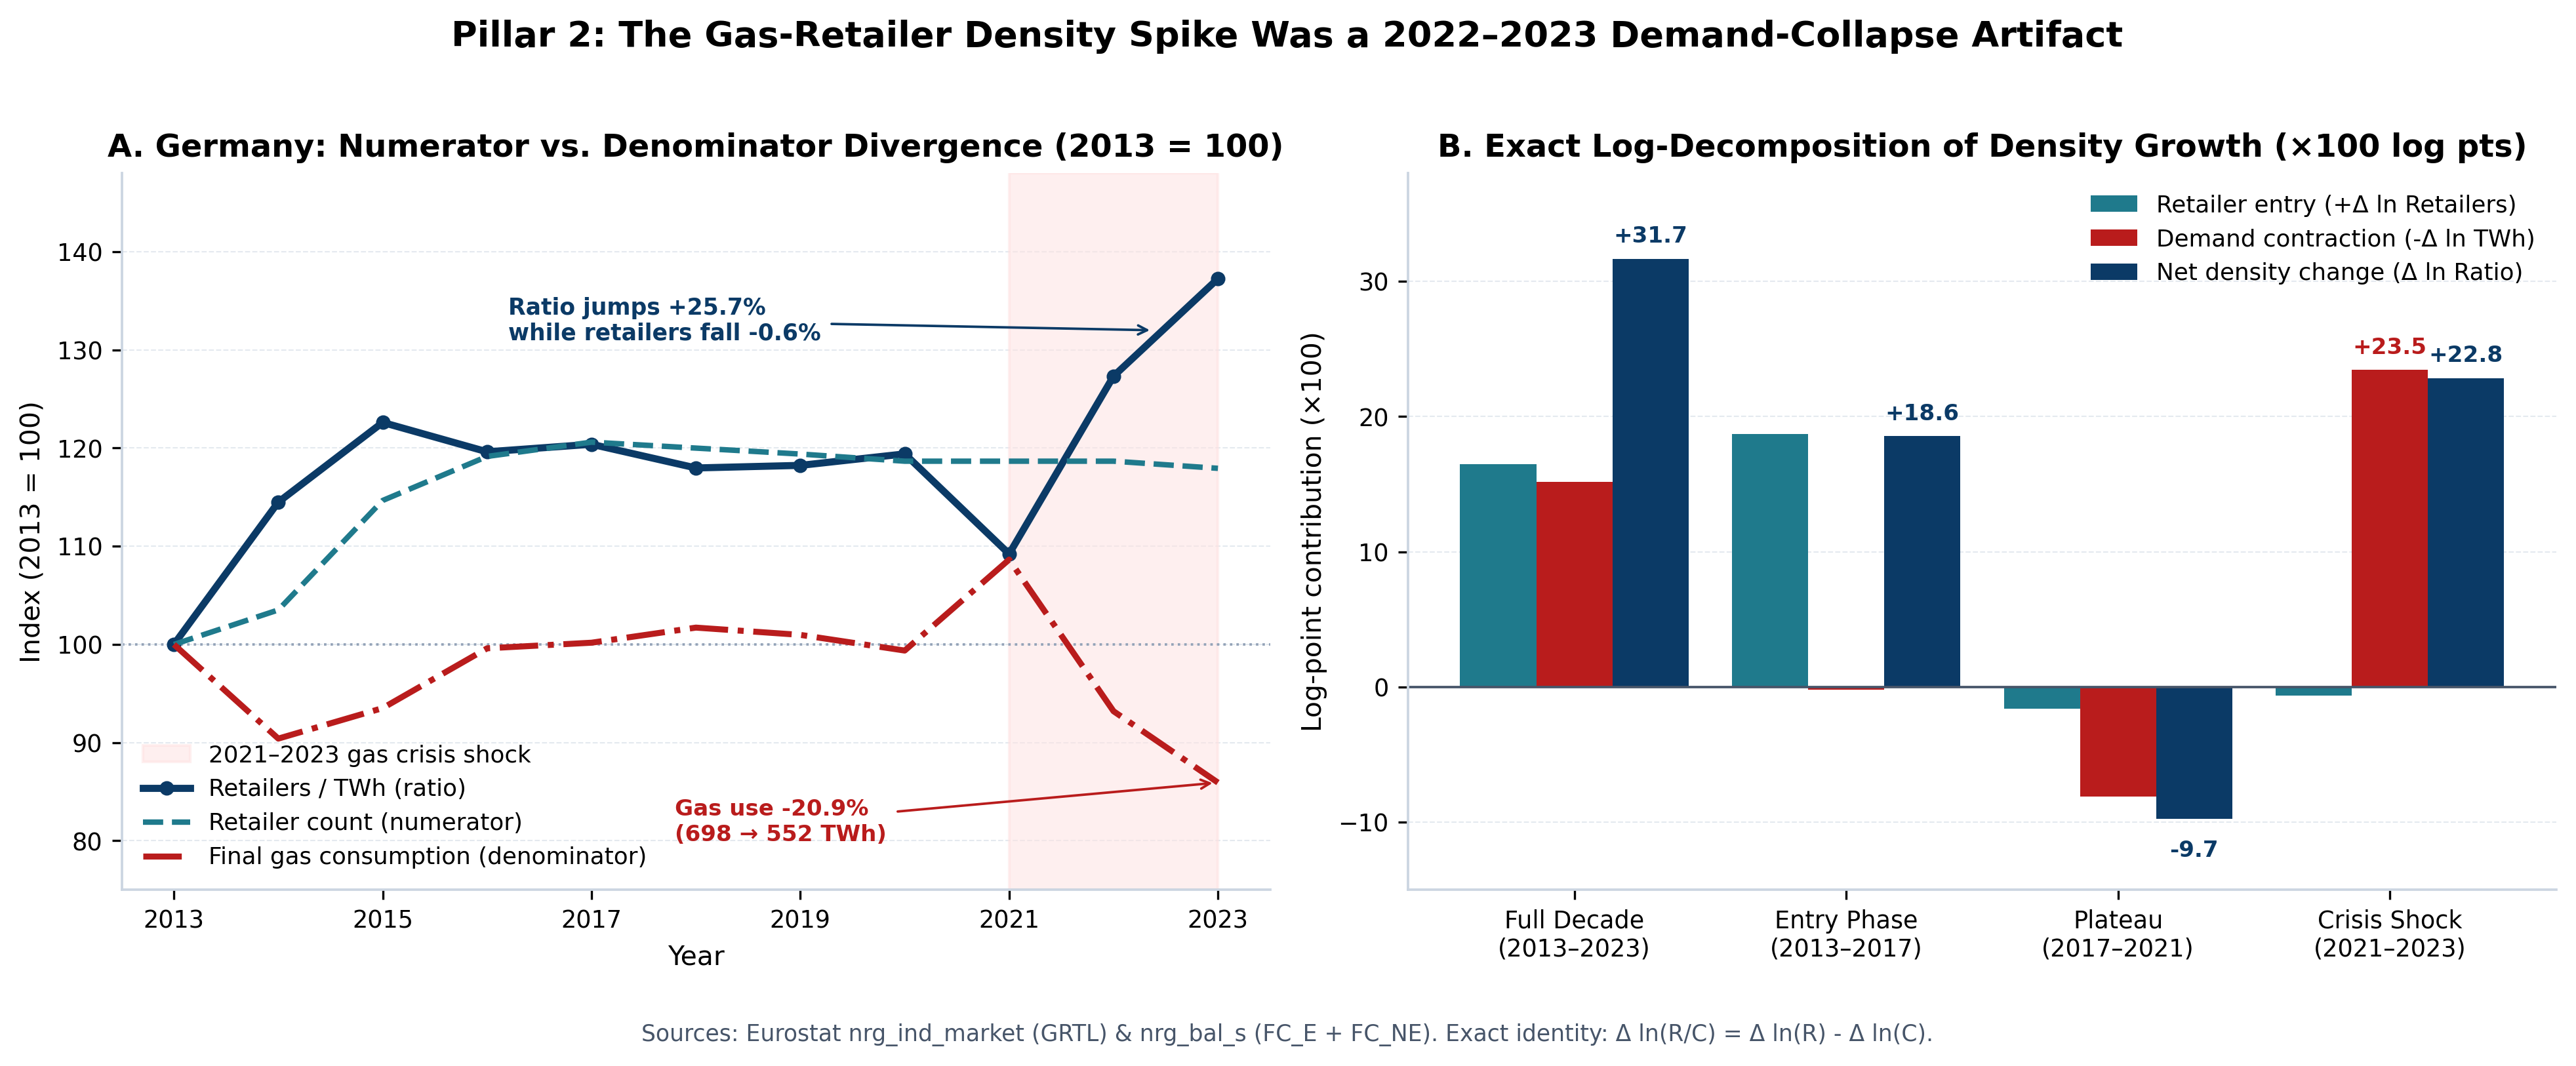
\includegraphics[width=0.98\textwidth]{fig2_gas_density_decomposition.png}
\caption{Pillar 2: Numerator-denominator divergence (Panel A) and exact log-decomposition across market regimes (Panel B) for German gas-retailer density.}
\label{fig:p2}
\end{figure}

\section{Pillar 3: Household Affordability and Tax-Wedge Regime Shift}

Despite electricity deconcentration and a \DERenElecTwentyThree\% renewable share, German households paid the highest nominal electricity rate in the Big-6 in 2023 (\DEElecEurTwentyThree~EUR/kWh; \DEElecPpsTwentyThree~PPS/kWh; Table~\ref{tab:big6_2023}). Figure~\ref{fig:p3} decomposes this surge into two policy regimes. Abolishing the EEG renewables surcharge slashed Germany's electricity tax wedge from \DEElecTaxTwentyOne\% in 2021 to \DEElecTaxTwentyThree\% in 2023, yet ex-tax energy and network charges rose from \DEElecExTaxTwentyOne~to \DEElecExTaxTwentyThree~EUR/kWh, pushing all-in bills higher. Household gas prices rose concurrently from \DEGasEurTwentyOne~to \DEGasEurTwentyThree~EUR/kWh.

\begin{figure}[ht]
\centering
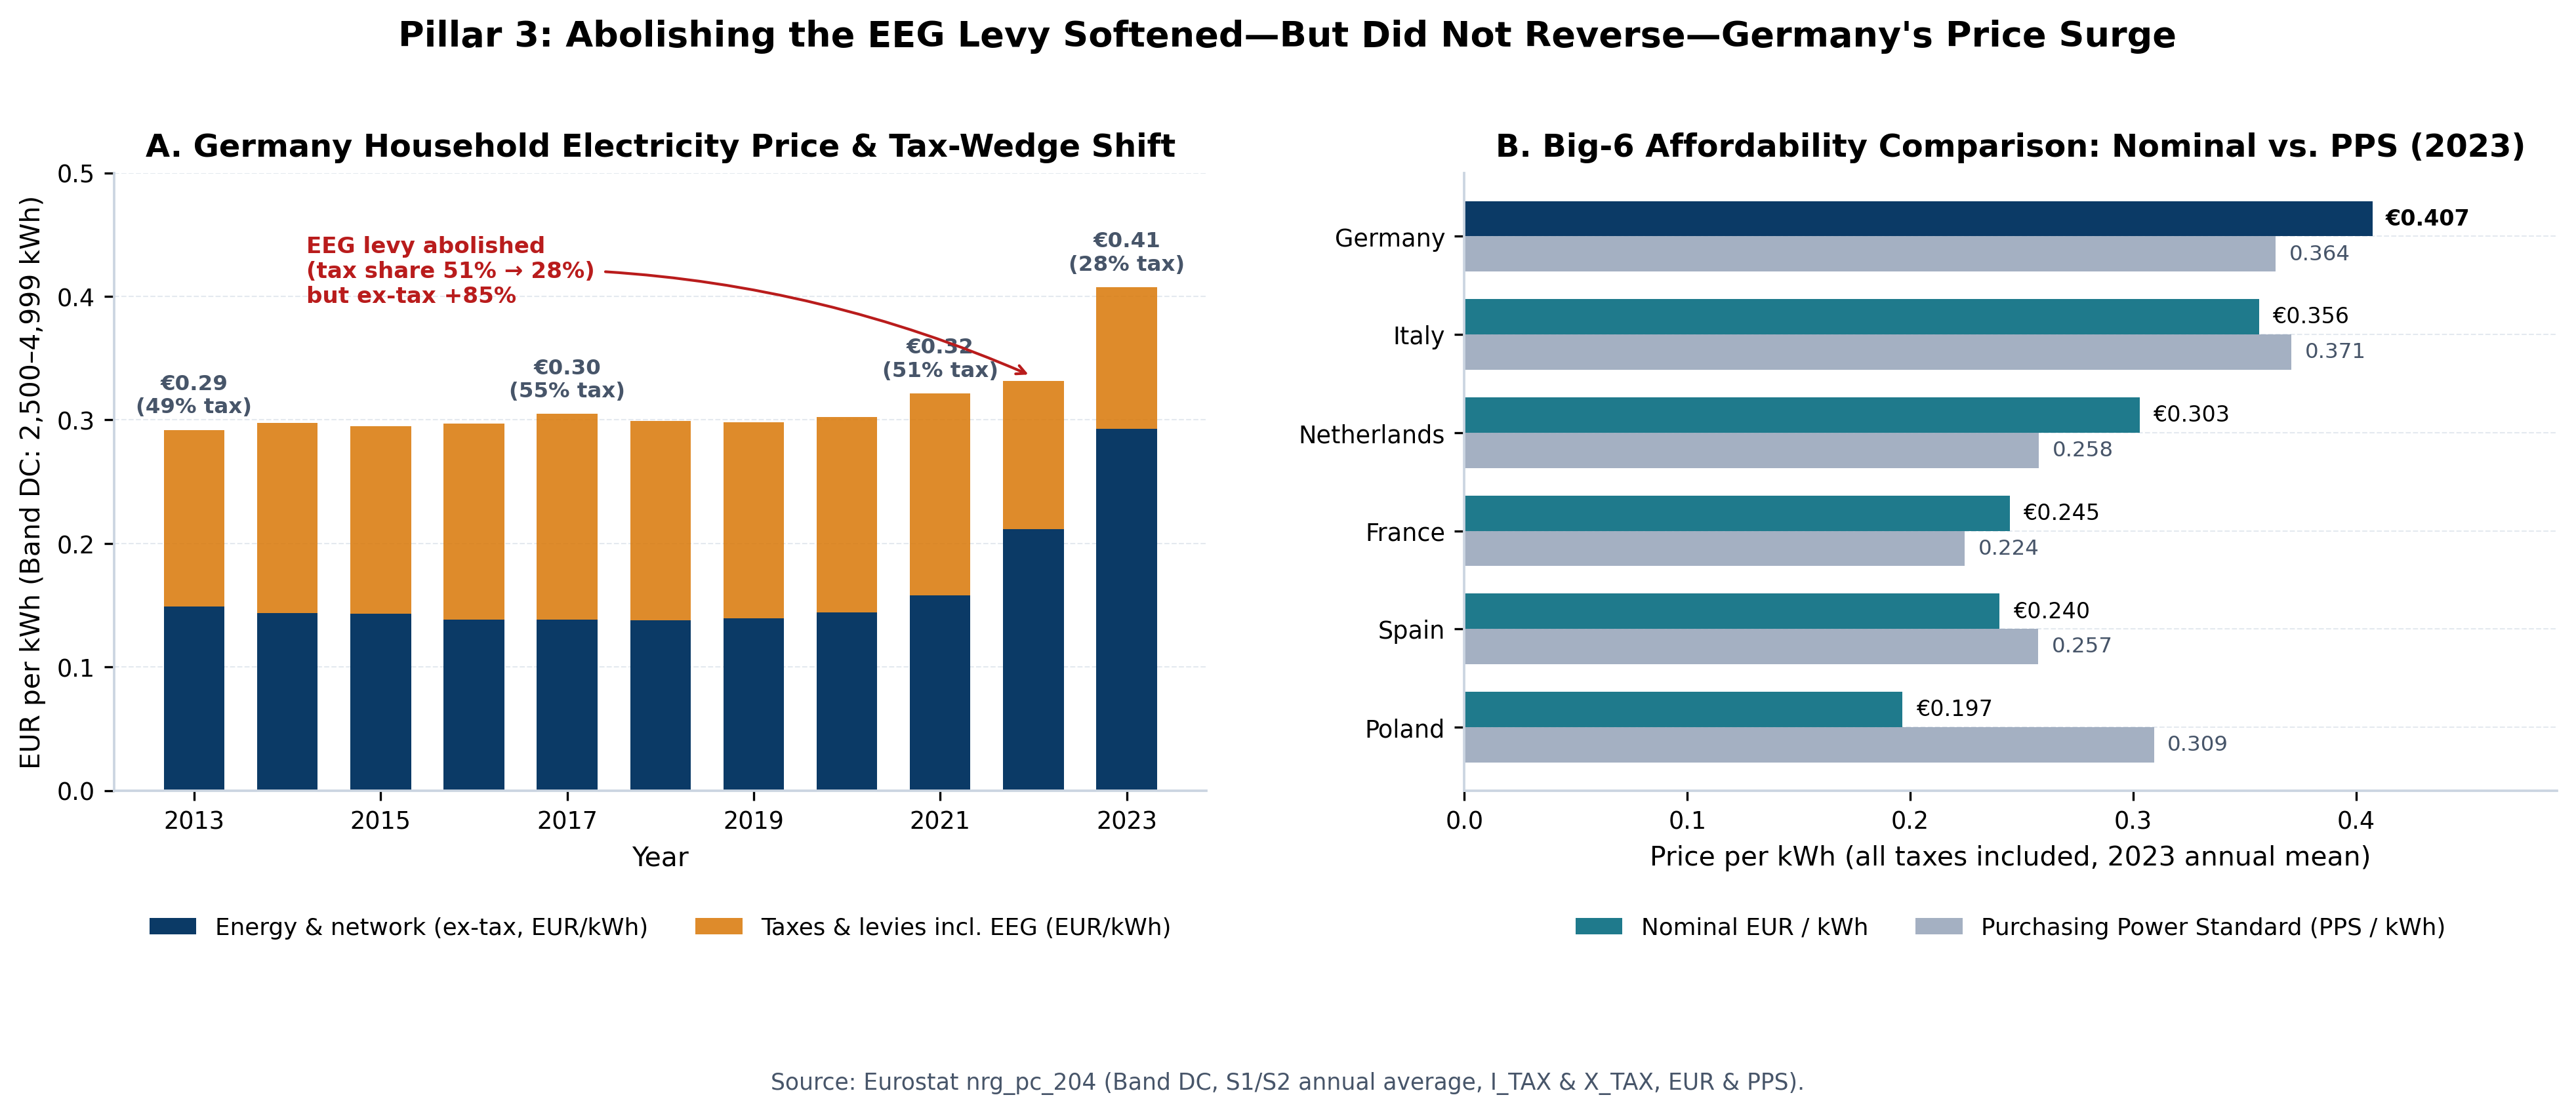
\includegraphics[width=0.98\textwidth]{fig3_affordability_tax_wedge.png}
\caption{Pillar 3: Germany's household electricity tax-wedge shift (Panel A) and Big-6 nominal vs.\ purchasing-power-adjusted electricity prices in 2023 (Panel B). Source: Eurostat \texttt{nrg\_pc\_204}.}
\label{fig:p3}
\end{figure}

\begin{table}[ht]
\centering
\caption{Europe's Big-6 markets in 2023: market structure, prices, and low-income thermal stress}
\label{tab:big6_2023}
\small
\begin{tabular}{@{}lrrrrrr@{}}
\toprule
Country & Gen. $\ge 5\%$ & Ren. Elec. & Gas Ret. $\ge 5\%$ & Elec. EUR & Elec. PPS & Low-Inc. Warm \\
\midrule
Germany & 57.1\% & 51.9\% & 13.3\% & 0.407 & 0.364 & 14.3\% (+6.5 pp) \\
Italy & 33.0\% & 38.9\% & 46.3\% & 0.356 & 0.371 & 21.6\% (+4.6 pp) \\
Netherlands & 30.0\% & 46.4\% & 78.0\% & 0.303 & 0.258 & 21.6\% (+14.0 pp) \\
France & 78.9\% & 30.3\% & 70.1\% & 0.245 & 0.224 & 25.1\% (+9.6 pp) \\
Spain & 49.8\% & 56.9\% & 70.1\% & 0.240 & 0.257 & 34.3\% (+6.6 pp) \\
Poland & 34.5\% & 25.8\% & 74.4\% & 0.197 & 0.309 & 9.8\% (+1.6 pp) \\
\bottomrule
\end{tabular}
\end{table}


\section{Pillar 4: Social Cohesion Stress Test and Panel Econometrics}

Because Germany experienced an EU-SILC methodological break in 2020, we evaluate the energy-crisis social stress test from 2021 to 2023. Inability to keep homes adequately warm (\texttt{ilc\_mdes01}) more than doubled in Germany from \DEWarmTotalTwentyOne\% (EU-27 rank \#\DEWarmTotalRankTwentyOne~of~27) to \DEWarmTotalTwentyThree\% (rank \#\DEWarmTotalRankTwentyThree~of~27), crossing \emph{above} the EU-27 median (\EUWarmTotalMedTwentyThree\%; Figure~\ref{fig:p4}). Among low-income households ($<60\%$ median income), thermal deprivation rose from \DEWarmLowIncTwentyOne\% to \DEWarmLowIncTwentyThree\%, and utility bill arrears increased from \DEArrearsLowIncTwentyOne\% to \DEArrearsLowIncTwentyThree\%. Even so, Germany's absolute low-income energy poverty stayed below Spain, France, Italy, and the Netherlands.

\begin{figure}[ht]
\centering
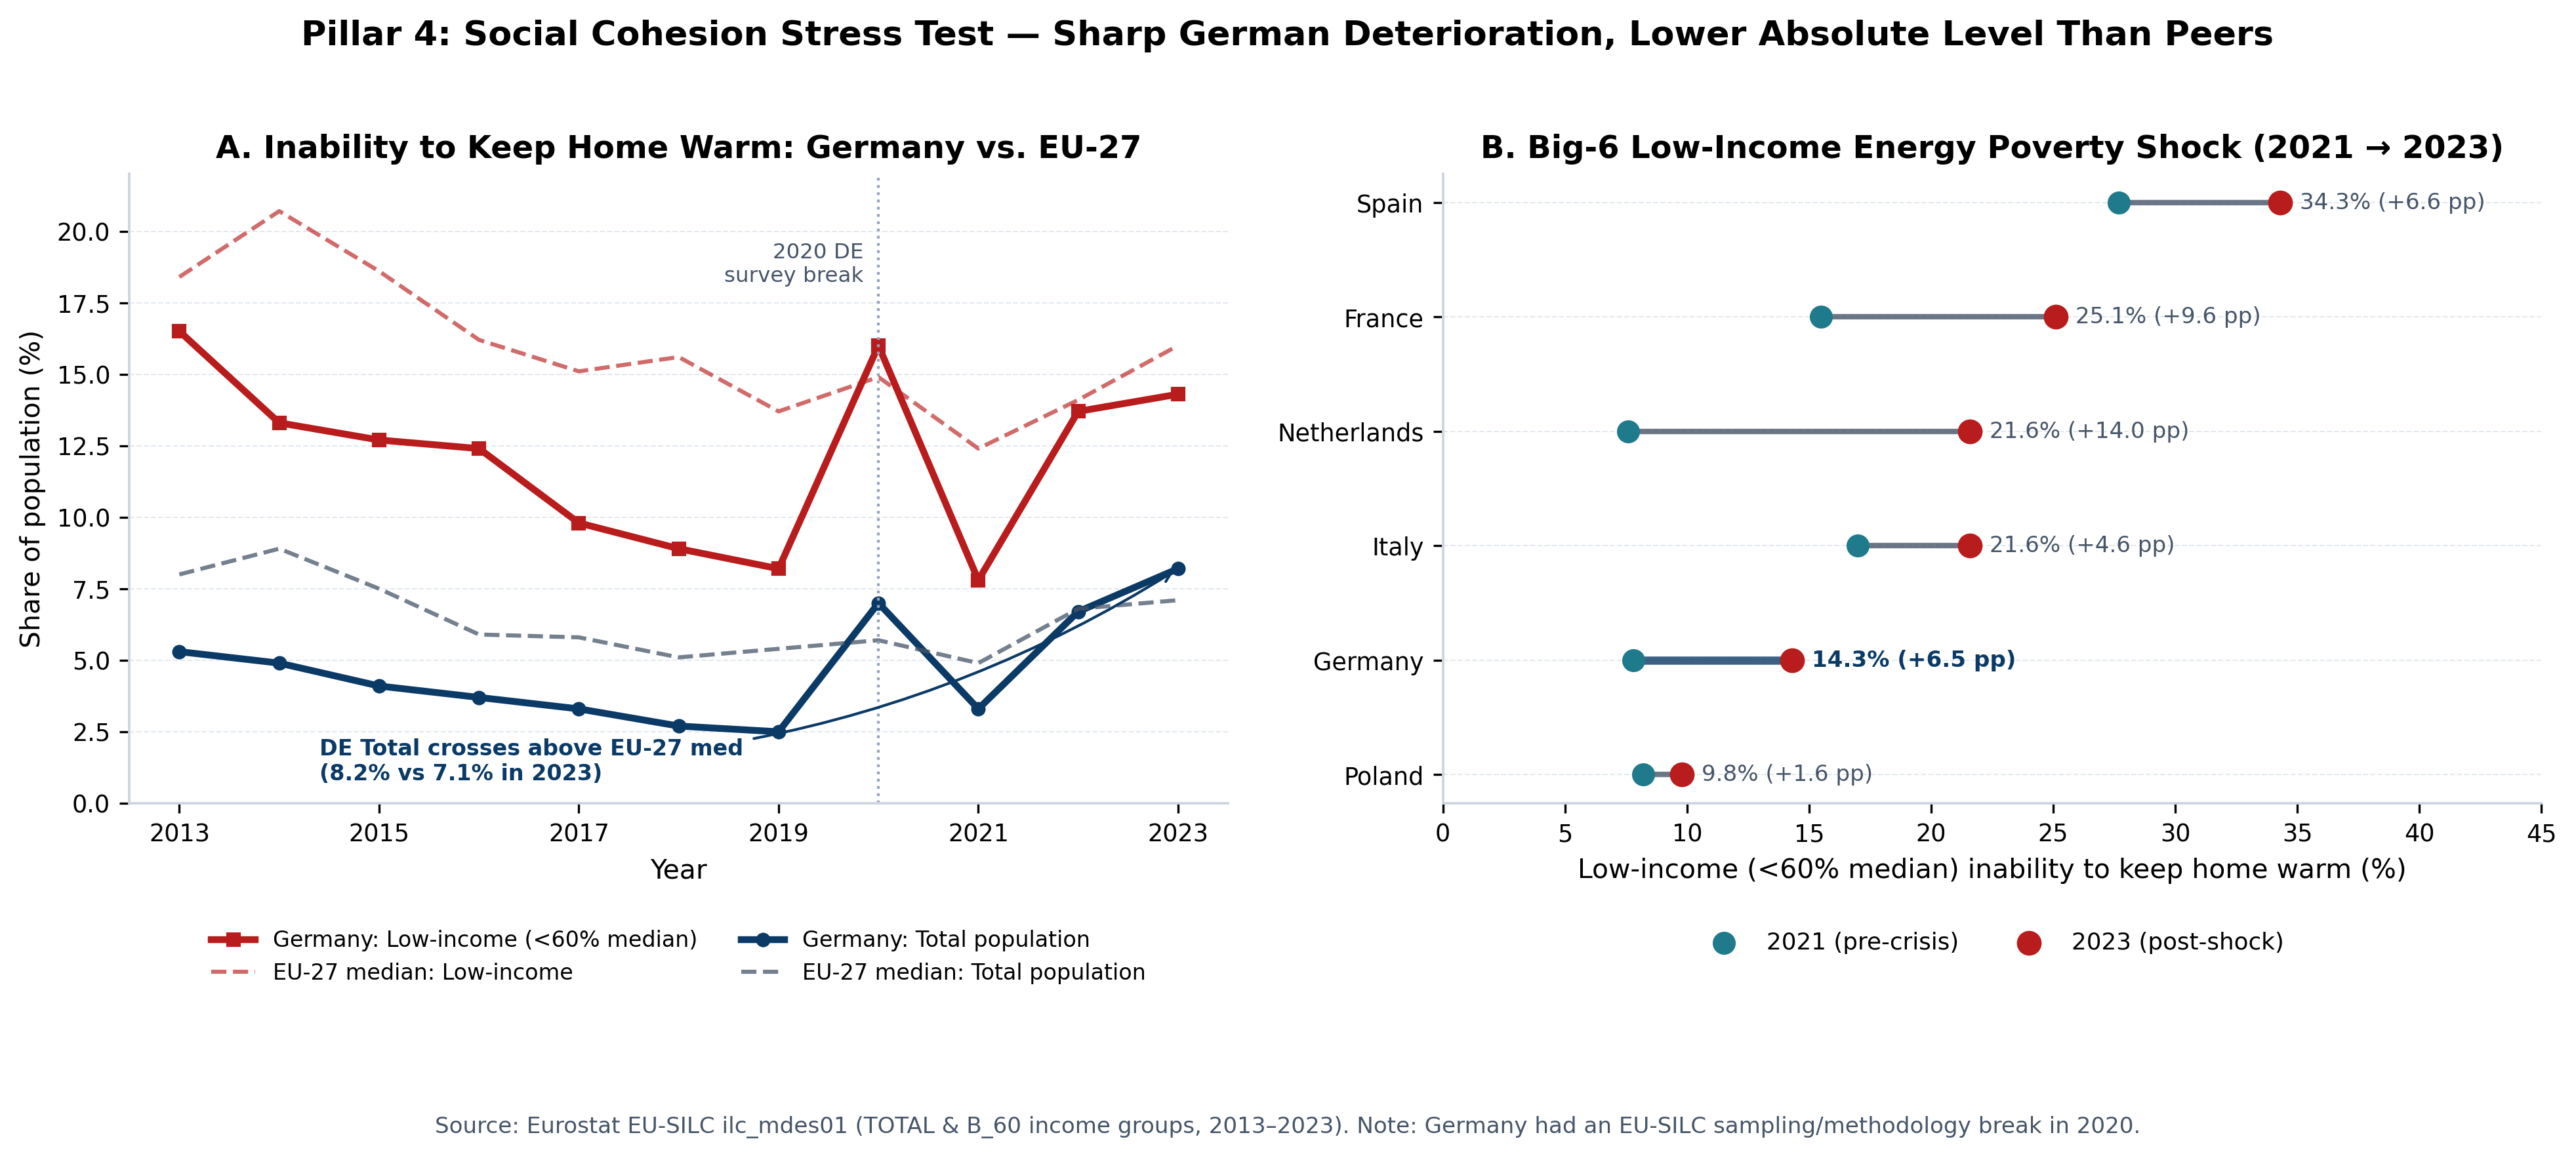
\includegraphics[width=0.98\textwidth]{fig4_social_cohesion_stress_test.png}
\caption{Pillar 4: Inability to keep home adequately warm in Germany vs.\ EU-27 medians (Panel A) and Big-6 low-income shock from 2021 to 2023 (Panel B). Source: Eurostat \texttt{ilc\_mdes01}.}
\label{fig:p4}
\end{figure}

Finally, Table~\ref{tab:twfe_models} and Figure~\ref{fig:p5} evaluate seven two-way fixed effects panel specifications (country and year fixed effects, country-clustered standard errors) against a strict pre-registered stability gate requiring 100\% leave-one-country-out sign preservation, $\le 50\%$ coefficient drift, and a 95\% confidence interval excluding zero. Models M1--M3 pass every test: within-country renewable electricity growth associates strongly with lower generation concentration ($\hat{\beta}=\MOneCoef$, within $R^2=\MOneWithinR$), and higher generation concentration associates with modestly higher PPS electricity prices ($\hat{\beta}=\MThreeCoef$, $p=\MThreePval$). Conversely, direct within-country regressions of thermal energy poverty on prices or concentration (M4--M6)—as well as the legacy v2 gas-density check (M7)—fail the gate.

\begin{table}[ht]
\centering
\caption{Two-way fixed effects panel associations with strict leave-one-out (LOO) stability gate}
\label{tab:twfe_models}
\resizebox{\textwidth}{!}{%
\begin{tabular}{@{}lrrrrrrl@{}}
\toprule
Model & Coef. & SE & 95\% CI & Within $R^2$ & $N$ & LOO $\le 50\%$ & Gate \\
\midrule
M1: Gen. conc. $\sim$ Ren. elec. (All) & -0.5330 & 0.2018 & [-0.928, -0.138] & 0.071 & 359 & 34/34 & \textbf{PASS} \\
M2: Gen. conc. $\sim$ Ren. elec. (EU-27) & -0.5390 & 0.2528 & [-1.034, -0.044] & 0.064 & 291 & 27/27 & \textbf{PASS} \\
M3: Elec. PPS $\sim$ Gen. conc. (EU-27) & 0.0007 & 0.0003 & [0.000, 0.001] & 0.032 & 291 & 27/27 & \textbf{PASS} \\
M4: Warmth (Tot) $\sim$ Elec. PPS & 8.9166 & 11.4073 & [-13.441, 31.274] & 0.008 & 297 & 25/27 & FAIL \\
M5: Warmth (Low-inc) $\sim$ Gas PPS & 32.6051 & 32.8292 & [-31.739, 96.949] & 0.012 & 264 & 22/24 & FAIL \\
M6: Warmth (Tot) $\sim$ Gen. conc. & 0.0240 & 0.0435 & [-0.061, 0.109] & 0.004 & 291 & 24/27 & FAIL \\
M7: Legacy v2 (Gas density $\sim$ Gen.) & 0.0026 & 0.0101 & [-0.017, 0.022] & 0.001 & 326 & 25/30 & FAIL \\
\bottomrule
\end{tabular}}
\end{table}


\begin{figure}[ht]
\centering
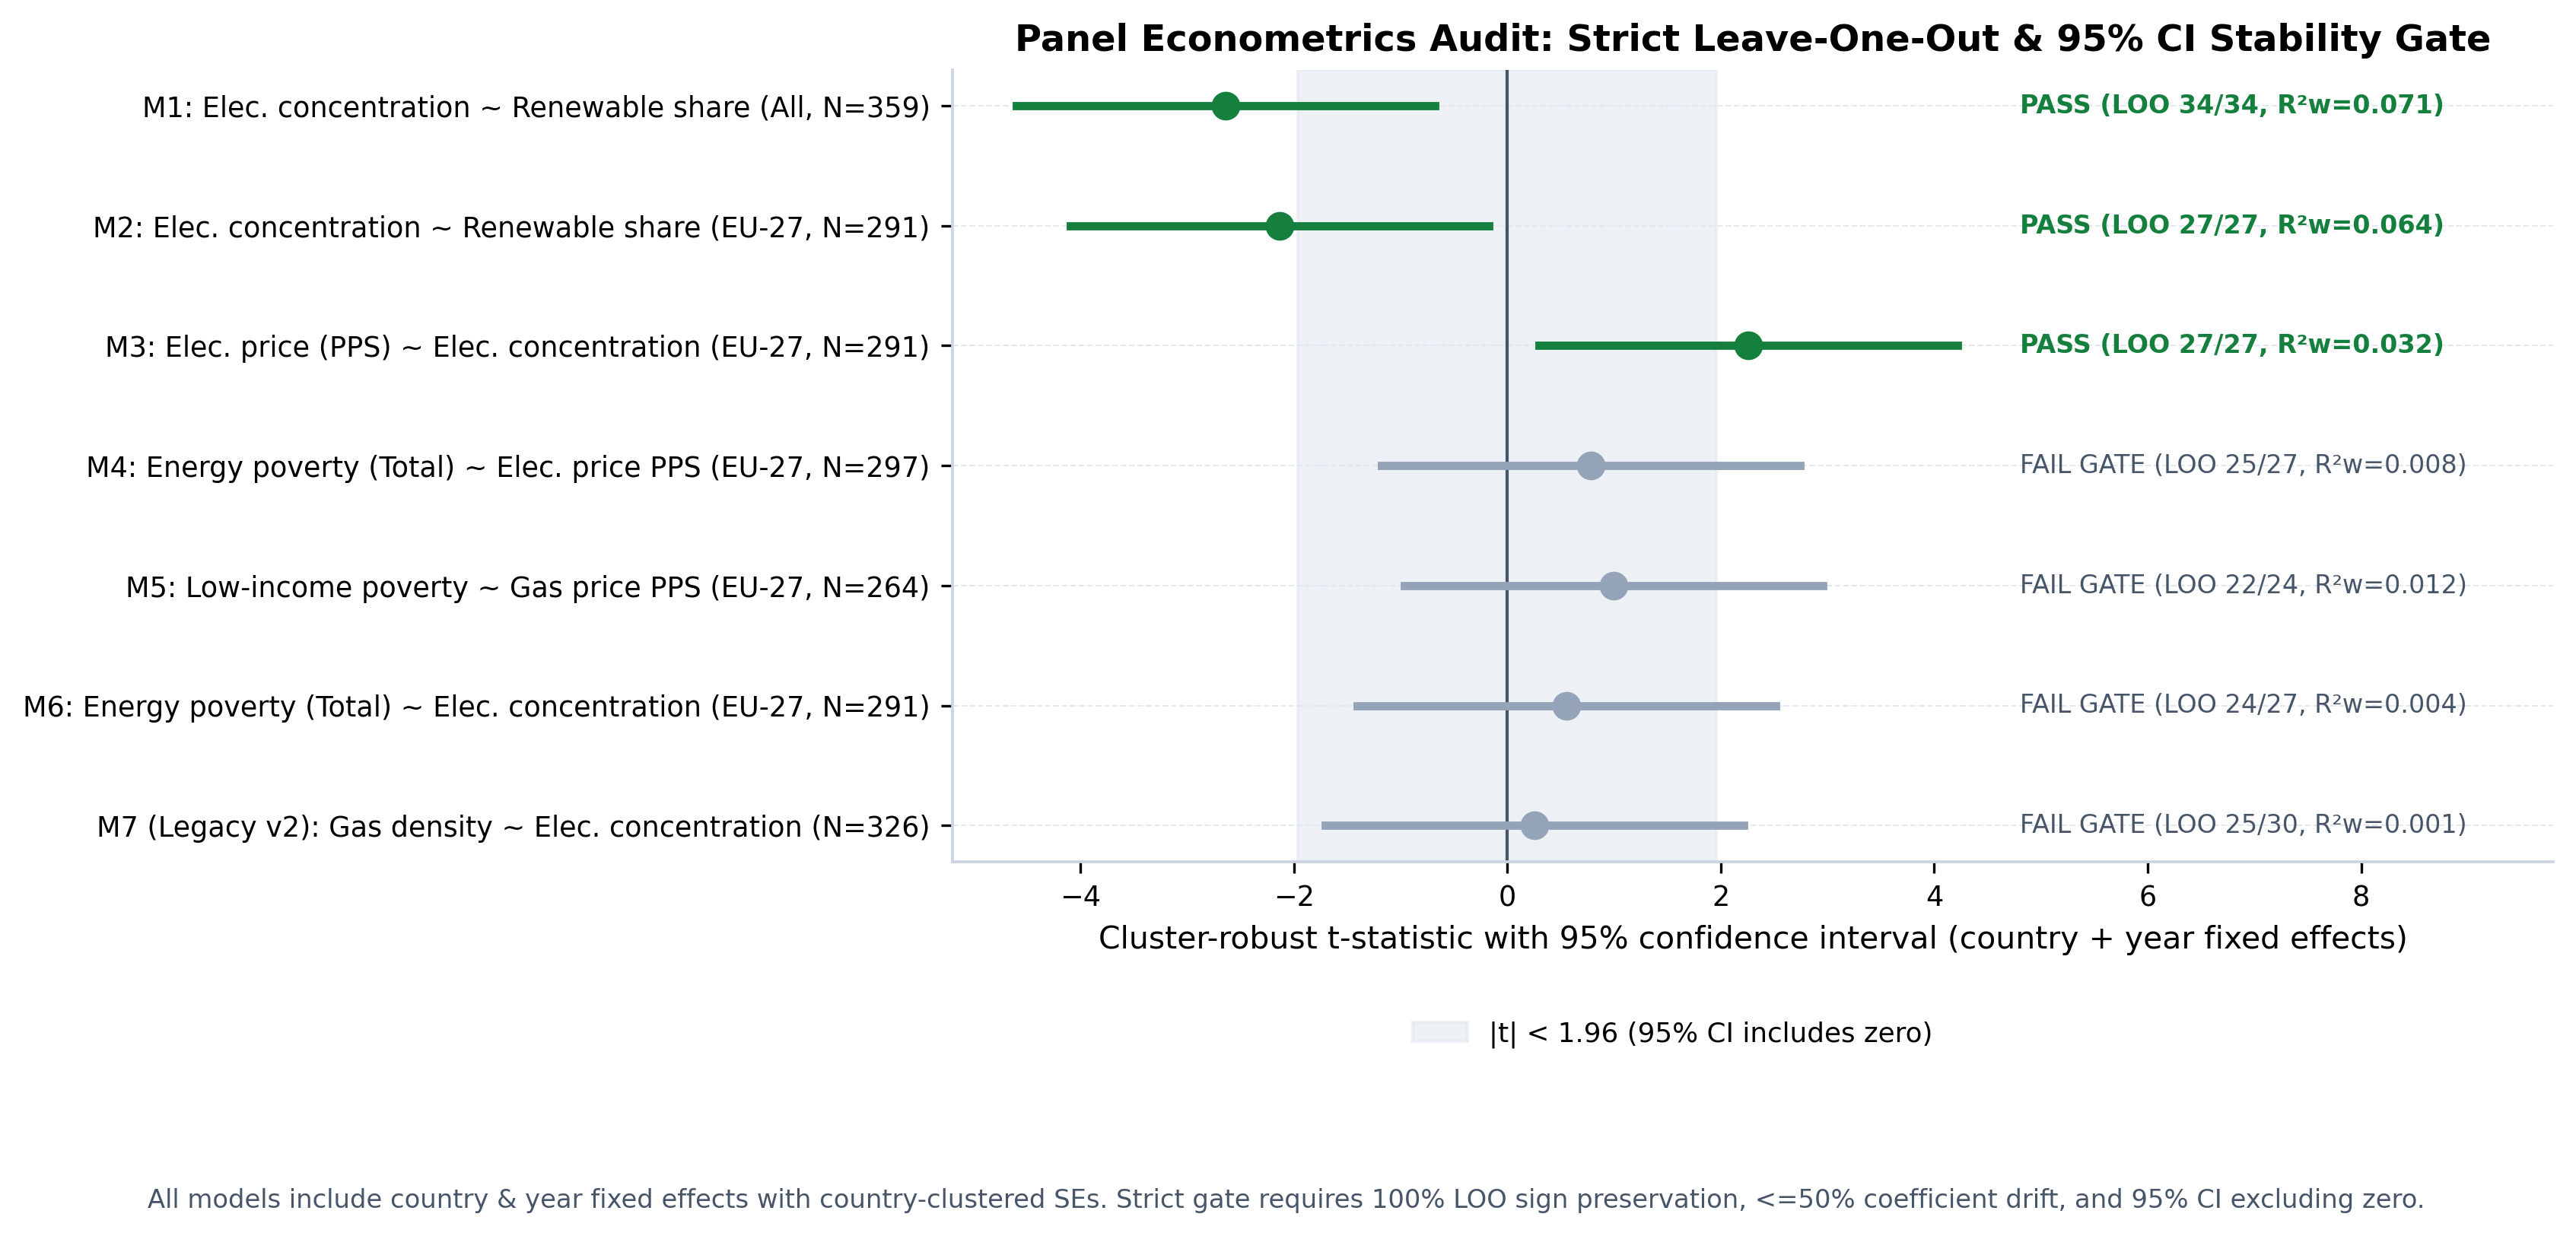
\includegraphics[width=0.98\textwidth]{fig5_twfe_stability_gate.png}
\caption{Cluster-robust $t$-statistics and 95\% confidence intervals across all seven two-way fixed effects specifications evaluated under the strict leave-one-out stability gate.}
\label{fig:p5}
\end{figure}

\section{Conclusion}

Germany's Energiewende reshaped electricity generation concentration through rapid renewable deployment, and its gas retail landscape remains the least concentrated among Europe's Big-6 economies. Yet the 2021--2023 crisis proves that market structure and renewable share alone do not automatically insulate households from acute price and thermal-deprivation shocks. Sustaining social cohesion through the energy transition requires pairing competitive market monitoring (using cohort-controlled, concentration-based metrics rather than crisis-distorted ratios) with targeted, income-indexed household protection.

\bibliographystyle{apalike}
\bibliography{references}

\end{document}
